\documentclass{article}

\usepackage{cancel}
\usepackage{amsmath}
\usepackage[includehead,nomarginpar]{geometry}
\usepackage{graphicx}
\usepackage{amsfonts} 
\usepackage{verbatim}
\usepackage{mathrsfs}  
\usepackage{lmodern}
\usepackage{braket}
\usepackage{bookmark}
\usepackage{fancyhdr}
\usepackage{romanbarpagenumber}
\usepackage{minted}
%\usepackage{subfig}
\usepackage[italian]{babel}
%\usepackage{float}
%\usepackage{wrapfig}
%\usepackage[export]{adjustbox}
\allowdisplaybreaks

\setlength{\headheight}{12.0pt}
\addtolength{\topmargin}{-12.0pt}
\graphicspath{ {../Immagini/} }

\hypersetup{
    colorlinks=true,
    linkcolor=black,
}

\newsavebox{\tempbox} %{\raisebox{\dimexpr.5\ht\tempbox-.5\height\relax}}


\makeatother

\numberwithin{equation}{subsection}
\newcommand{\tageq}{\tag{\stepcounter{equation}\theequation}}
\AtBeginDocument{%
  \renewcommand{\figurename}{Fig.}
}
\fancypagestyle{link}{\fancyhf{}\renewcommand{\headrulewidth}{0pt}\fancyfoot[C]{Sorgente del file LaTeX disponibile al seguente link: \url{https://github.com/00Darxk/Reti-di-Calcolatori/}}}

\begin{document}

\title{%
    \textbf{Reti di Calcolatori}  \\ 
    \large Appunti delle Lezioni di Reti di Calcolatori \\
    \textit{Anno Accademico: 2024/25}}
\author{\textit{Giacomo Sturm}}
\date{\textit{Dipartimento di Ingegneria Civile, Informatica e delle Tecnologie Aeronautiche \\
Università degli Studi ``Roma Tre"}}

\maketitle
\thispagestyle{link}

\clearpage


\pagestyle{fancy}
\fancyhead{}\fancyfoot{}
\fancyhead[C]{\textit{Reti di Calcolatori - Università degli Studi ``Roma Tre"}}
\fancyfoot[C]{\thepage}
\pagenumbering{Roman}

\tableofcontents

\clearpage
\pagenumbering{arabic}

\section{Esercitazione 23/10/24}

\subsection{Rete Bridge con Cicli}

Si considera una rete locale IEEE 802.3 di topologia seguente:

\begin{figure}[H]%
    \centering%
    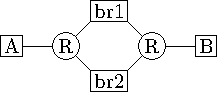
\includegraphics[scale=1.25]{rete_bridge_cicli.pdf}%    
\end{figure}

Sono presenti due repeater R, e due computer A e B. Le connessioni avvengono solo su cavi utp, ``Unshielded Twisted Pair'', si suppone che questi 
bridge numerati 1 e 2, non siano in grado di realizzare lo spanning tree. Quindi tutta la rete, compreso il ciclo, è attiva. Si suppone che tutte 
le porte dei bridge siano pienamente attive. 
Si suppone che i bridge siano appena stati accesi, quindi i loro filtering database siano vuoti. 

Il primo evento in questa rete locale è l'invio di un pacchetto da A e B. 

\subsubsection*{Domanda 1}

Determinare quanti pacchetti circolano nella rete dopo l'invio del singolo pacchetto:

Questo pacchetto \verb|(A->B)| arriva ad entrambi i bridge \verb|bridge 1| e \verb|bridge 2|, che hanno un filtering database vuoto, per cui lo mandano su tutte le 
porte attive. Poiché il repeater può inviare ricevere un pacchetto alla volta si considera che il pacchetto del primo bridge arrivi per primo al repeater, nella 
contesa del dominio di collisione. Si considerano i due pacchetti copiati dai due bridge \verb|(A->B)'|, il primo, e \verb|(A->B)'|, il secondo. 
Ma il repeater invia il pacchetto ricevuto su tutte le direzioni, quindi oltre ad arrivare a B, arriva anche alla porta destra dell'altro bridge, che invia la sua copia 
del pacchetto dalla porta sinistra. Questo pacchetto incontra il repeater della sotto-rete A e viene ripetuto su tutte le porte del repeater. Quindi questo pacchetto 
oltre a raggiungere A viene inviato sulla porta sinistra dell'altro bridge, e si ripete la sequenza, per entrambi i bridge. 

Quindi in questa situazione le copie del pacchetto \verb|(A->B)'| viene inviato continuamente in un ciclo antiorario, mentre \verb|(A->B)''| segue il percorso 
orario. 

\subsubsection*{Domanda 2}

Determinare cosa succeeded al filtering database di \verb|bridge 1| e \verb|bridge 2|:

Ogni volta che il pacchetto copiato raggiunge un bridge, considera la porta da cui è arrivato la nuova posizione della stazione A, così per entrambi i bridge. 
Quindi la sua posizione nel filtering database cambia continuamente. 

\subsubsection*{Domanda 3}

Determinare il comportamento dei bridge all'invio di un pacchetto \verb|(B->A)|: 

Se il pacchetto arriva ad entrambi i bridge quando la stazione A si trova nel 
filtering database sulla porta destra, il pacchetto non viene inviato ad A. Se solo uno presenta la stazione A alla porta sinistra, una singola copia raggiunge A. 
Se entrambi presentano la stazione A alla porta sinistra, questa riceve due volte il pacchetto. 


Dati questi problemi non si accetta di avere un ciclo in una rete neanche per un tempo transitorio, poiché può saturare la rete ed impedire ai pacchetti necessari a 
passare. Gli algoritmi per determinare lo spanning tree sono molto conservativi, e prima di effettuare l'algoritmo interrompono il transito di tutti i pacchetti. 
\clearpage

\subsection{Effetto dello Store \& Forward sulla Latenza}

Si considera una rete mostrata nella figura seguente, dove A e B sono computer e S1 e S2 sono switch. Dove i cavi ethernet sono utp, ed il ritardo di propagazione 
è trascurabile. Si suppone che le schede di rete utilizzate sono tutte a 10 Mb/s. 

Questo disegno mostra cosa avviene sulla rete mentre è in funzione, rispetto al tempo:

\begin{figure}[H]%
    \centering%
    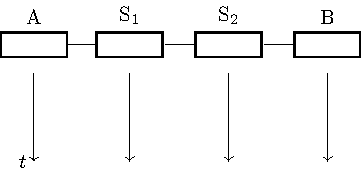
\includegraphics{effetto_store_forward.pdf}%
\end{figure}

Il computer deve spedire un file di 100000 bit a B, suddividendolo in 100 pacchetti. Si suppone che il trasferimento inizi all'istante $t=0$, e si suppone di trascurare 
gli header e l'IPG. Si suppone che la rete sia a completa disposizione del trasferimento dei file, che gli switch non operino in modalità ``cut-through''. Si suppone che non 
siano utilizzati riscontri di alcun tipo. 

\subsubsection*{Domanda 1}

Completa il diagramma temporale riportato al di sotto della figura con la rete, mostrando la sequenza dell'invio dei pacchetti dai vari componenti:

\begin{figure}[H]%
    \centering%
    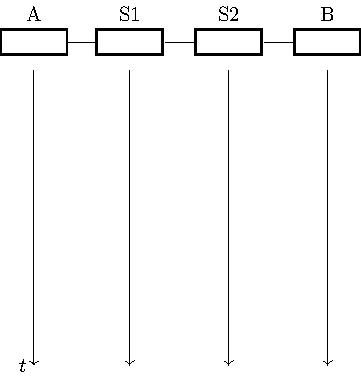
\includegraphics{effetto_store_forward_domanda_1.pdf}%
\end{figure}

Ad ogni istante lo switch ha un pacchetto in ricezione su una porta, ed un pacchetto in trasmissione sulla seconda porta. 

Per inviare un singolo pacchetto sulla rete si impiega un tempo $t_i$:

\begin{equation}
    t_i=\displaystyle\frac{100000\,\mathrm{bit}/100\,\mathrm{pk}}{10^7 \mathrm{bit/s}}=10^{-4}\mathrm{s/pk}
\end{equation}

In caso il ritardo non sia trascurabile, ogni segmento viene traslato verso il basso di questo ritardo. 

\subsubsection*{Domanda 2}

In quale istante tutti i bit sono arrivati a B:


Il primo pacchetto viene ricevuto completamente ad un tempo $3t_i$, poiché deve passare attraverso tre spazi intermedi, dopo il quale i pacchetti 
arrivano ogni $t_i$, e rimanendo 99 pacchetti, l'ultimo arriverà al tempo $102t_i$. 
\begin{equation}
    T=102\,t_i
\end{equation}


\subsubsection*{Domanda 3}

Determinare una formula generale per risolvere ogni problema di questo tipo con $n$ pacchetti ed $m$ switch:

Ogni switch aggiunge un altro stadio alla trasmissione, quindi aumenta il tempo di un fattore $t_i$, da aggiungere al numero di pacchetti totali:
\begin{equation}
    T=(n+m)\cdot t_i
\end{equation}

\begin{figure}[H]%
    \centering%
    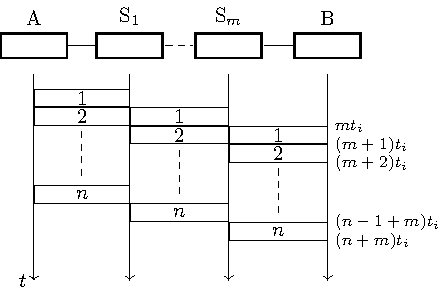
\includegraphics{effetto_store_forward_domanda_3.pdf}%
\end{figure}

\subsubsection*{Domanda 4}

Determinare una formula generale che tenga conto di ritardi sul primo, sul secondo, o sul terzo filo: 

In caso di un ritardo su un certo filo, questo rappresenta il collo di bottiglia del sistema, e quindi il tempo totale ne risentirà 
considerevolmente. Il tempo in cui il primo bit del primo pacchetto arriva $T_1$ è dato dal tempo di attraversamento di ogni filo, quindi è $T_1=3t_i+t_i^{\mathrm{r}}$, 
dove $t_i^{\mathrm{r}}$ rappresenta il tempo di ritardo su di un filo. Tutti gli altri $n-1$ pacchetti arriveranno ad intervalli di $t_i+t_i^{\mathrm{r}}$, quindi il tempo di arrivo 
dell'ultimo di $n$ pacchetti trasmessi è:
\begin{equation}
    T=T_1+(n-1)\cdot (t_i+t_i^{\mathrm{r}})=(n+2)\cdot t_i+nt_i^{\mathrm{r}}
\end{equation}

%% TODO img disegno

\subsubsection*{Domanda 5}

Si suppone di poter aumentare la connessione ad una banda di 100 Mb/s, ma questo aumento è possibile solo su uno dei tre fili, utilizzando 
una doppia scheda su di un filo. Anche se il tempo di trasmissione di un pacchetto in uno dei fili diventa il decimo: $t^*_i=t_i/10$, il 
resto dei fili rimane alla stessa banda, quindi rappresenta il collo di bottiglia del sistema. Quindi l'aumento di banda su un singolo filo non influisce sulla 
diminuzione del tempo necessario per tutti i pacchetti, ma solo per il primo $T_1=2t_i+t_i^*$. Tutti gli altri 99 pacchetti arrivano alla destinazione ogni $t_i$, come per il 
problema originario:
\begin{equation}
    T=T_1+99t_i=101t_i+t_i^*
\end{equation}

\begin{figure}[H]%
    \centering%
    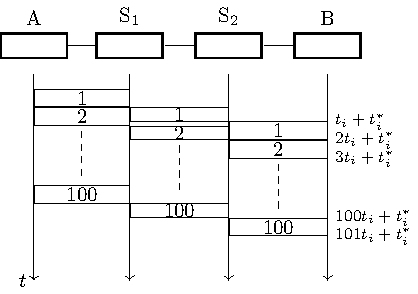
\includegraphics{effetto_store_forward_domanda_5.pdf}%
\end{figure}

\subsection{Learning nei Bridge}

\subsubsection*{Domanda 1}

Si considera un bridge b1 con quattro porte \verb|eth0|, \verb|eth1|, \verb|eth2| e \verb|eth3|, a cui sono collegati quattro computer a, b, c, d:
\begin{figure}[H]%
    \centering%
    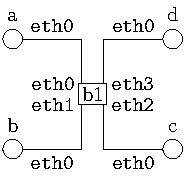
\includegraphics{singolo_bridge.pdf}%   
\end{figure}

Nella rete transitano 
cinque pacchetti in sequenza, inviati dopo che il precedente è giunto a destinazione: 
\begin{itemize}
    \item t$_1$: \verb|(a->b)|;
    \item t$_2$: \verb|(b->a)|;
    \item t$_3$: \verb|(c->d)|;
    \item t$_4$: \verb|(c->d)|;
    \item t$_5$: \verb|(d->a)|. 
\end{itemize}

Descrivere il contenuto del filtering database di B1, dopo ciascun pacchetto, e specificare le porzioni di rete in cui i diversi pacchetti sono visibili. 

Il pacchetto t$_1$ viene ricevuto dalla porta \verb|eth0|, quindi viene assegnata ad A nel filtering database, e viene inviato su tutte le altre le porte. 
Il pacchetto t$_2$ viene ricevuto dalla porta \verb|eth1|, questa porta viene associata al computer B, e sapendo dove si trova A, lo invia solamente sulla porta \verb|eth0|.
I pacchetti t$_3$ e t$_4$ effettuano un procedimento analogo a t$_1$ e t$_2$, sulle porte \verb|eth2| e \verb|eth3|. 
All'arrivo del pacchetto t$_5$, il bridge conosce l'intera topologia della rete. 

Ma il filtering database non è statico, e viene dimenticato in intervalli di tempo prestabiliti, oppure se uno dei computer viene connesso ad un'altra porta 
e ne riceve un pacchetto. Quindi se uno di questi pacchetti arriva dopo che è stato resettato il filtering database, ricomincia il processo di learning. 

\subsubsection*{Domanda 2}

Si considera la seguente topologia di rete ad albero, con tre bridge b1, b2, e b3, e tre computer a, b e c: 
\begin{figure}[H]%
    \centering%
    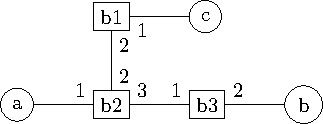
\includegraphics{albero_bridge.pdf}%
\end{figure}

Nella rete vengono trasmessi tre pacchetti, inviati in tre istanti di tempo successivi:
\begin{itemize}
    \item t$_1$:\verb|(a->c)|;
    \item t$_2$:\verb|(c->a)|;
    \item t$_3$:\verb|(b->a)|. 
\end{itemize}

Descrivere il filtering database per all'invio di ciascun pacchetto, e specificare in quali porzioni di rete i pacchetti sono visibili:

All'invio del primo pacchetto tutti i filtering database sono vuoti, quindi il pacchetto t$_1$ viene inviato su ogni porzione della rete. Dopo il suo invio, il 
bridge b2 ha sulla porta 2 la stazione a, il bridge b3 ha sulla porta 1 la stazione a, ed il bridge b1 la ha sulla porta 2. 
All'invio del pacchetto t$_2$, sia il bridge uno che due sanno dove si trova la stazione a, quindi il pacchetto viene prima inviato dalla stazione c a b1, poi da b1 
all'altro bridge b2, poi da b2 alla stazione di arrivo a. Alla fine della trasmissione i bridge uno e due hanno la stazione c rispettivamente sulla porta 1, e 2. 
All'invio dell'ultimo pacchetto t$_3$, entrambi i bridge b3 e b2 hanno la stazione a nel loro filtering database, quindi effettua un percorso da b a b3, a b2 fino ad a. 
Il bridge b2 e b3 conoscono la posizione della stazione b rispettivamente sulle porte 3 e 2. 


\subsubsection*{Domanda 3}

Considerando la stessa rete dell'esercizio seguente, come cambia il filtering database se i pacchetti precedenti vengono inviati nell'ordine:
\begin{itemize}
    \item t$_1$:\verb|(c->a)|;
    \item t$_2$:\verb|(b->a)|;
    \item t$_3$:\verb|(a->c)|. 
\end{itemize}

I primi due pacchetti vengono trasmessi su tutta la rete, mentre solo l'ultimo viene trasmesso solo sulle porte necessarie, dato che i bridge conoscono la posizione 
del destinatario. 
Dopo il primo pacchetto i bridge b1, b2 e b3, conoscono la posizione della stazione c, rispettivamente sulla porta 1, 2, 1. All'invio del secondo pacchetto analogamente 
conoscono la posizione della stazione b sulle porte, 2, 2, 2. Mentre all'invio dell'ultimo pacchetto i bridge b1 e b2 conoscono la posizione della stazione a sulle porte 
1 e 2. 
Rispetto alla domanda precedente, il bridge b3 ora conosce la posizione della stazione c, ma il bridge b3 non conosce la posizione della stazione a. 

\clearpage

\section{Esercitazione 13/11/24}

Lo spazio degli indirizzi viene rappresentato come un albero binario, etichettato sugli archi con un valore 0 o 1. L'arco che esce da un nodo verso 
il figlio sinistro viene etichettato come 0, mentre quello destro viene etichettato con un 1. 

In questa rappresentazione ad albero una foglia, a profondità 32 rappresenta un indirizzi, il suo cammino fino alla radice rappresenta tutti i 32 bit dell'indirizzo 
IPv4 corrispondente. 
Gli indirizzi sono in corrispondenza biunivoca con le foglie dell'albero. Una net in questa rappresentazione corrisponde ad un nodo che non è una foglia, 
infatti tutte le macchine in una stessa net hanno un certo cammino dalla radice ad un nodo in comune. Il sotto-albero radicato in questo nodo rappresenta tutti gli 
indirizzi appartenenti alla stessa net. 
Il suo prefisso è ottenuto completando questa net con tutti zeri, quindi è il cammino sempre verso sinistra in questo sotto-albero

%% TODO img, domande

\subsection{Domanda 3}

Come è possibile verificare che due net non abbiano indirizzi in comune?\\
Dati due nodi dell'albero, se il più basso antenato comune corrisponde ad uno dei nodi dell'albero, allora gli indirizzi non sono disgiunti, 
mentre se gli indirizzi non si sovrappongono %% TODO ??

\subsection*{Domanda 4}

Nella rappresentazione ad albero data una rappresentazione di una net A e la rappresentazione di una net B, come è possibile verificare che A e B siano il risultato 
esatto del ``subnetting'' di una terza net C?\\
Bisogna 

\subsection*{Domanda 5}

\end{document}